\section{Experimental Setup}
\label{sec:experimentalSetup}

Our evaluation compares six different continuous sensing methods: 

\begin{enumerate}
\setlength{\itemsep}{-3pt}  

\item \textbf{Always Awake}. Provides a baseline for the following methods in terms of event detection recall and precision.

\item \textbf{Duty cycling}. A software-only solution that checks sensor readings periodically and then puts the phone to sleep. This method can be implemented on any mobile device and does not require special hardware support.

\item \textbf{Sensor data batching}. A hardware extension to duty cycling method that matches the Always Awake method in terms of detection recall and precision, but is expected to consume less power.

\item \textbf{Activity detection}. Assumes hardware support for activity detection, specifically a step detector. Allows the exploration of the benefits of hardware-based activity recognition as a wake-up condition.

\item \textbf{Custom filter-based wake-up condition}. Assumes hardware support for the selection of a pre-defined data filter and customization of filter and wake-up parameters. Allows us to explore the benefits of filter customization.

\item \textbf{Oracle}, a hypothetical, ideal wake-up condition. The device only wakes up when there exists an event of interest to be recognized. Such a wake-up condition would achieve the same detection precision and recall as Always Awake, with the lowest possible energy consumption. The difference between the power consumption of this method and the method using custom filter-based wake-up conditions gives an upper bound on the potential benefits of fully configurable hardware, beyond limited data filter selection.

\end{enumerate}

We implement applications using these different sensing methods and use trace-based simulation for comparison. The rest of this section describes our trace collection methodology, the sensing applications that we have implemented, and the operation of our trace-based simulator.

%%  alternative implementations of
%% applications that perform continuous sensing.  We consider approaches that
%% assume that the phone is always-on, performs duty cycling, has access to
%% hardware that buffers sensor readings, provides an API that either lets
%% applications register for notifications based on pre-defined activity
%% recognition, and provides an API that lets applications specify custom wakeup
%% conditions by configuring pre-defined filters.

\subsection{Trace Collection}

We use traces in our evaluation because they help provide the same
input to the different sensing methods. To compare these methods, we
need ground truth about the occurrence and the timing of desired
events, such as steps taken. Annotating accelerometer traces collected
from human subjects with the ground truth is time-consuming and error
prone.

Instead, we used an AIBO ERA 210 robot dog (see Figure~\ref{fig:aibo})
to collect the ground truth about events and accelerometer traces for
our experiments. The robot performed a sequence of actions in a
course, and we logged these actions and the timestamps for the
beginning and the end of each action. This log represents the ground
truth for our experiments. We also logged the robot's acceleration by 
attaching a Google Nexus 4 to the back of the robot. The smartphone was 
used to run an application that kept the device continuously awake and 
recorded all the accelerometer readings. The accelerometer trace collected 
for each course is an ordered set of
accelerometer readings. Each reading contains the x, y and z
components of the acceleration vector and a timestamp indicating when
the reading was produced.

To get statistically significant results, the robot was programmed to run multiple different 
courses. In a course, the robot performed five different types of actions: standing idle, 
walking, sit-to-stand transitions, stand-to-sit transitions, and headbutts. We divided the 
courses into three different groups to cover an increasing amount of activity levels. Courses in 
groups 1, 2 and 3 spent 90\% , 50\% and 10\% of the time standing idle, respectively. The 
reminder of the time was allocated as follows: 73\% for walking, 24\% for transitions between 
sitting and standing, and 3\% for headbutts. Figure~\ref{fig:actionTimes} shows the average 
amount of time that each action is performed in each group, as a percentage of the average time 
taken to complete the course. This set-up allows us to experiment with detecting actions that 
are common, somewhat frequent, and rare. In total, the robot ran 18 different courses, 
partitioned as follows: 9 for the group 1, 6 for group 2 and 3 for group 3. We chose to run more 
course in groups 1 and 2 because of the lower activity levels compared to group 3. To eliminate 
bias, the list of actions was generated randomly for each course, based on the expected 
probabilities of each action occurring. Running each course generated a separate ground truth 
log of actions and an accelerometer trace.  

\begin{figure}[t]
	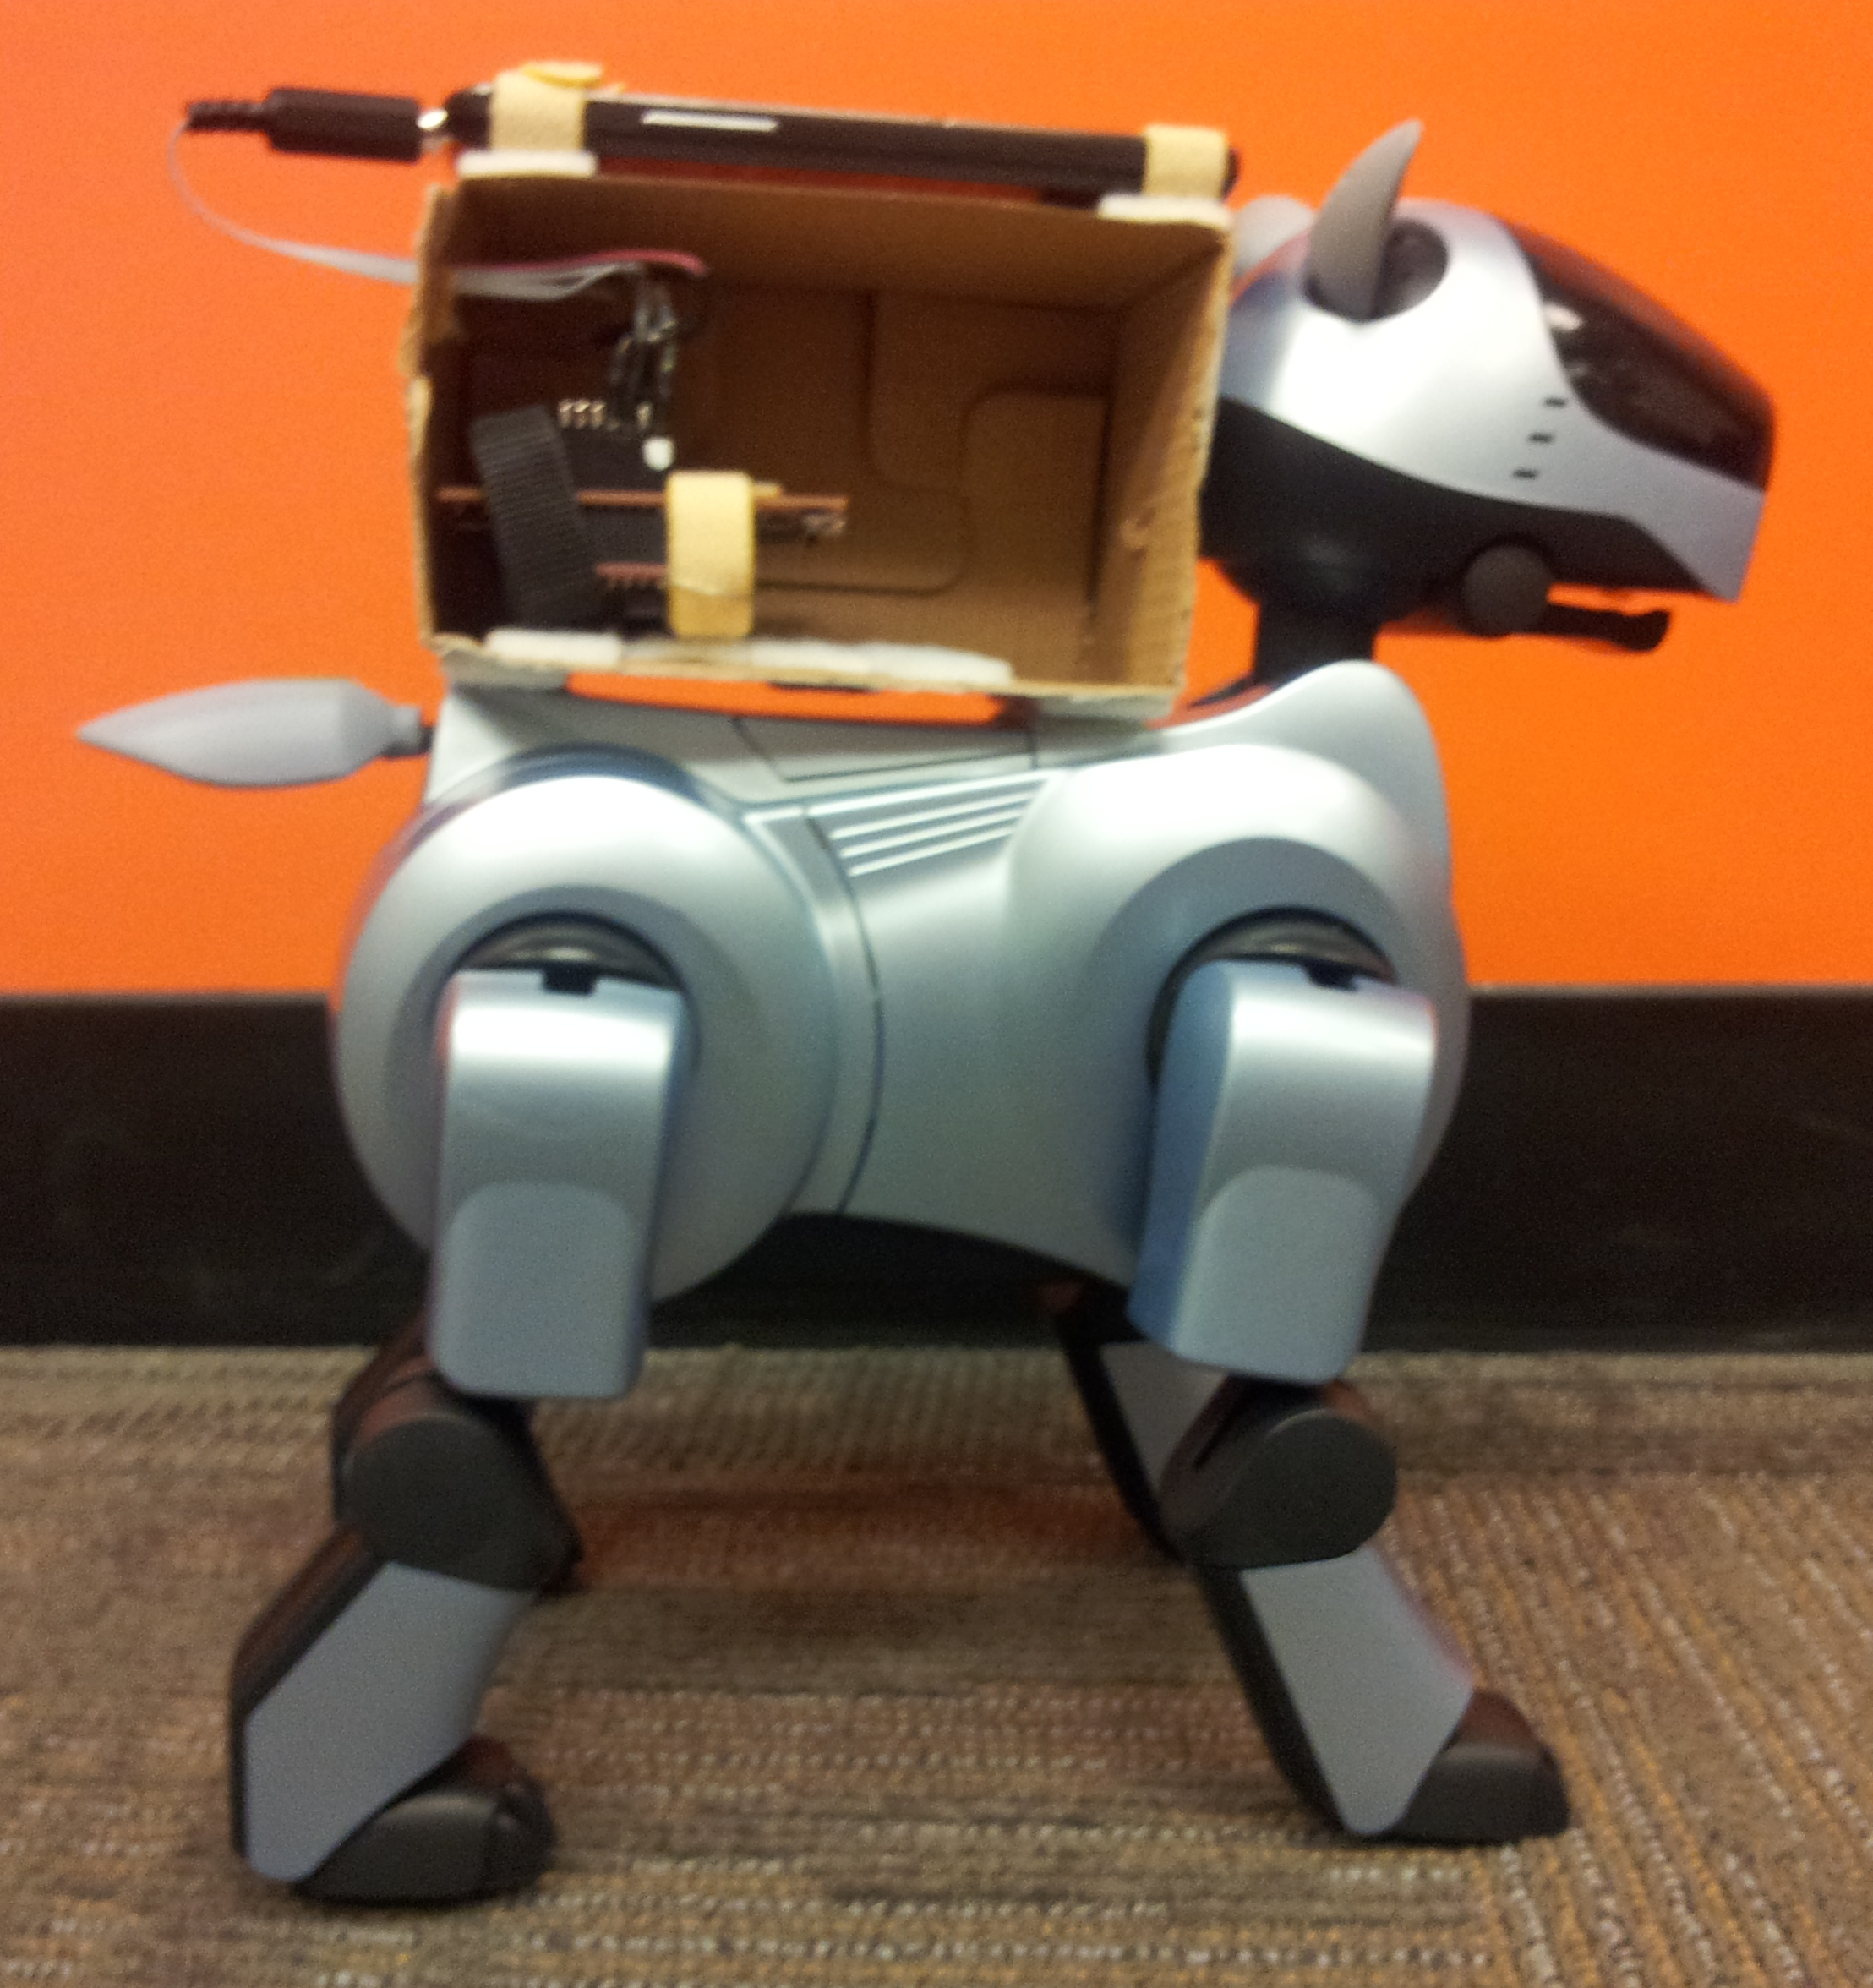
\includegraphics[width=8.5cm]{aibo_ers_210.jpg}
	\caption{AIBO ERS 210 robot used to collect the accelerometer traces}
	\label{fig:aibo}
\end{figure}

\begin{figure}[t]
	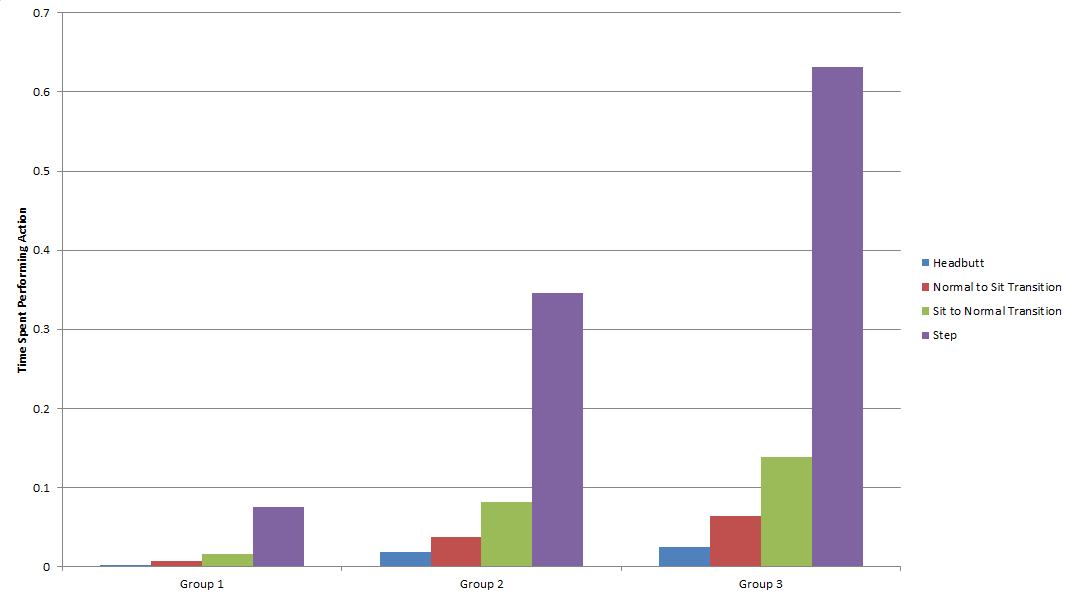
\includegraphics[width=8.5cm]{action_times.png}
	\caption{Percent time spent performing actions of specific types}
	\label{fig:actionTimes}
\end{figure}

\subsection{Applications}

The objective of this work is to match the recall and precision of the Always Awake approach while using less power. Our objective was not to build more accurate sensor-driven applications, but to lower the energy cost of running these kinds of algorithms. We present detection precision and recall metrics to demonstrate that the applications we used are doing a reasonable job, and are therefore legitimate choices to use in our experiments. Achieving perfect event of interest detection is not our objective. 

\todo[inline]{Ashvin: as stated, this sentences sounds like we carefully chose applications that would work well for us (thus introducing bias), and they do "okay" with our approach.
consider dropping or rewording this entire sentence. e.g., it is not clear what point the sentence is making. The sentence (achieving perfect ..) could also be dropped}

For our microbenchmarks, we implemented three applications:

The \textbf{Step} application counts how many steps the robot takes when it walks. It's algorithm is based on the human step detection algorithm proposed by Ryan Libby in \cite{libbyFootstepDetection}. The application takes in raw accelerometer readings and applies a low-pass filter on the x-axis acceleration. It then searches for local maxima in the filtered x-axis acceleration. Local maxima between $2.5\:m/s^2$ and $4.5\:m/s^2$ are detected as steps, given that no other steps were detected within the last 100 ms.

The \textbf{Headbutt} application works very similarly to the Steps application. The major differences are that it uses the y-axis acceleration and that it searches for local minima between $-3.75\:m/s^2$ and $-6.75\:m/s^2$.

The \textbf{Sit-Stand} application monitors changes in acceleration due to gravity on the y and z axes to determine the orientation of the device. If the z-axis (up-down relative to the dog) acceleration is between $9 m/s^2$ and $11 m/s^2$, and the acceleration on the y-axis (front-back relative to the dog) is between $-1 m/s^2$ and $1 m/s^2$, the device is in a horizontal position and the robot is assumed to be in a standing posture, as shown in Figure \ref{fig:aibo}. Similarly, if the z-axis acceleration is between $7.5 m/s^2$ and $9.5 m/s^2$, and the acceleration on the y-axis is between $3.5 m/s^2$ and $5.5 m/s^2$, the device is in an angled position and the robot is assumed to be in a sitting posture. The application detects transitions by looking for posture changes.

\begin{figure}[t]
	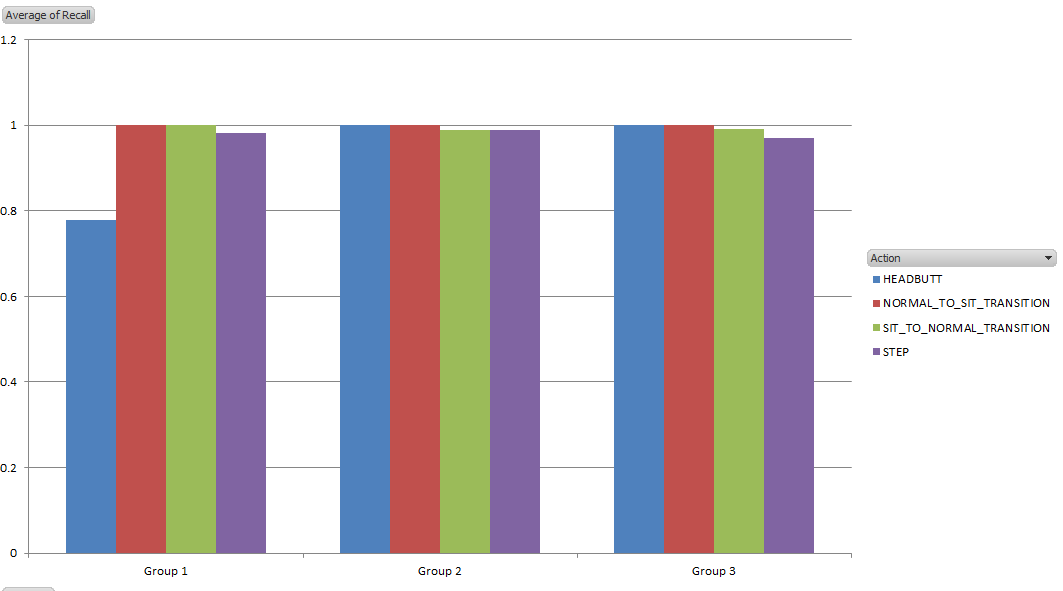
\includegraphics[width=8.5cm]{aa_recall_by_group.png}
	\caption{Always Awake: Recall by Group}
    	\label{fig:aaRecallByGroup}
\end{figure}


\begin{figure}[t]
	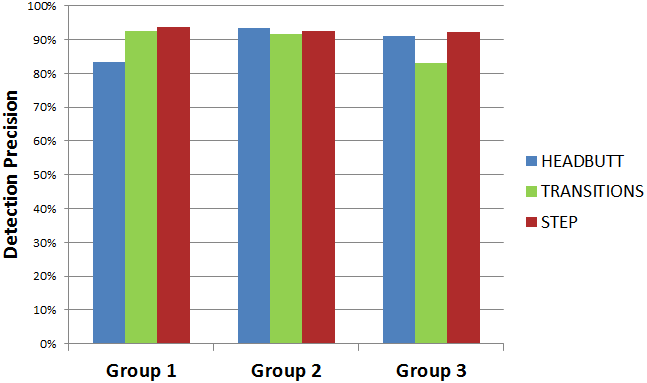
\includegraphics[width=8.5cm]{aa_precision_by_group.png}
	\caption{Always Awake: Detection Precision by Group}
    	\label{fig:aaPrecisionByGroup}
\end{figure}

Figure \ref{fig:aaRecallByGroup} shows the average recall for all applications when executing on a phone that is kept always on.  The 
Headbutt and Stand-Sit applications detected all the events of interest, achieving a recall of 100\%. The Steps application achieved a 
recall above 97\% for all three groups. Figure \ref{fig:aaPrecisionByGroup2} shows the detection precision of each of the events of 
interest averaged over the traces in each group. For all cases, the applications achieved a detection precision above 82\%.

%%	We usethese applications for evaluating always-on operation, duty cycling,
%%	and batching. The activity detection and wake-up condition sensing
%%	methods require programming the low-power processor. To evaluate these
%%	methods, we developed a variant of each application that runs three
%%	types of filters on the low-power processor: 1) simple threshold, 2)
%%	exponential moving average, and 3) FFT. The low power processor wakes
%%	up the phone when these filters indicate that an event of interest has
%%	been detected. The application then runs its FFT algorithms on the
%%	main processor to eliminate false alarms, i.e., events that where
%%	misidentified by the low-power processor.

%% \todo[inline]{This needs to be expanded.

%%For each application, describe the parameters that provided the best results for each filter.   Perhaps %%this can be done using a table.   You can point out that these parameters where obtained experimentally %%and that we perform a sensitivity analysis in the next section.}

\subsection{Trace-based Simulator}

The objective of our simulations is to compare the different sensing methods in terms of detection recall, wakeup precision and power consumption for various usage scenarios. To do this, the simulator is used to process the collected traces using each of the sensing methods listed at the beginning of this section. Also, the simulator allows us to explore the parameter configuration space for each of the more complex sensing methods (duty cycling, batching, custom wake-up conditions).

Each simulation run takes several inputs:

\begin{itemize}
\setlength{\itemsep}{-3pt}  

\item An accelerometer trace. These files were collected on the smart phone attached to the robot during each of the courses.

\item A ground truth log file. These files were generated by the robot while performing each of the courses.

\item The sensing method to be used.

\item A set of parameters for the sensing method used.

\end{itemize}

\begin{figure}[t]
	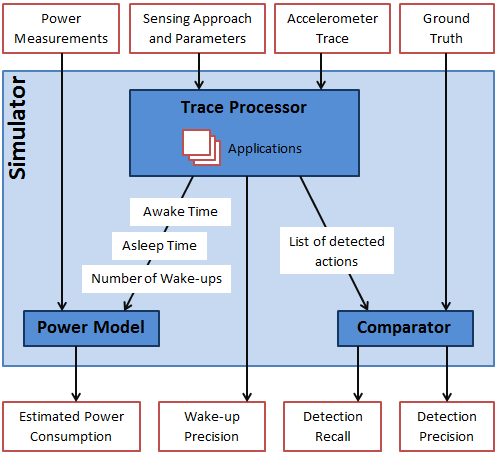
\includegraphics[width=8.5cm]{simulator.png}
	\caption{Overview of the Simulator and its three main modules}
	\label{fig:simulator}
\end{figure}

Figure \ref{fig:simulator} shows an overview of the simulator. The simulator is made up of three main modules: a \textit{Trace Processor}, a \textit{Comparator} and a \textit{Power Consumption Model}. 

The \textit{Trace Processor} simulates both the low-power and the main processor. It takes the accelerometer trace and handles the readings one at a time, similar to the way a mobile device would receive accelerometer readings in real-time, as they are produced by the sensor. Based on the sensing method used and its parameters, the \textit{Trace Processor} determines when the device should wake-up and what accelerometer readings should be sent to the running application(s). This enables the \textit{Trace Processor} to output the amount of time the device is awake and asleep, the total number of wake-ups and the wake-up precision (defined below). Also, the \textit{Trace Processor} runs the detection applications and produces a list of actions detected by the applications and the times when each of the actions occurred.

The \textit{Comparator} takes as inputs the file containing ground truth data about the actions performed by the robot during the course and the list of detected actions that is produced by the \textit{Trace Processor}. It compares the two lists based on action timestamps and determines detection recall and precision.

Finally, the \textit{Power Consumption Model} module uses metrics from the \textit{Trace Processor} to estimate the average power consumption of the system. The input metrics are awake and asleep times of the device, and the total number of wake-ups. The \textit{Power Consumption Model} estimates power consumption based on the power consumption measurements presented in Subsections \ref{subsec:nexus} and \ref{subsec:sensorBoard}.

Overall, the main metrics outputted by the simulator are:


\todo[inline]{Move Table 3 after Table 2. What about Group 2? Why not present Precision as well.
It is hard to gauge absolute power numbers. Why not present the ratio power over power in always awake}

\begin{itemize}
\setlength{\itemsep}{+5pt}  

\item Detection recall of event of interest

$Recall = \dfrac{Correctly\:detected\:actions}{Number\:of\:actions\:in\:ground\:truth}$

$Recall = \dfrac{True\:Positives}{True\:Positives + False\:Negatives}$\linebreak[2]


\item Detection precision of event of interest

$Precision = \dfrac{Correctly\:detected\:actions}{Number\:of\:detected\:actions}$

$Precision = \dfrac{True\:Positives}{True\:Positives + False\:Positives}$\linebreak[2]


\item Estimated average power consumption over the duration of the trace


\item Wake-up precision

$Wakeup\:Precision = $

$ = \dfrac{Number\:of\:wakeups\:with\:detected\:actions}{Number\:of\:wakeups}$\linebreak[2]

\end{itemize}



\subsection{Discussion}
\label{subsec:discussion}

Since we are mainly interested in actions that would normally be
performed by humans, we configured the robot to perform actions with
similar acceleration signatures. A walking robot has a similar
acceleration signature as its human counterpart, though at a lower
intensity. The headbutts are meant to represent very infrequent human
actions such as falling. We found that robot stance transitions
between the normal and sitting postures are very similar in their
acceleration signature to humans sitting down and standing up.

Rather than using a trace-based simulator, it is possible to run live
experiments with a robot because it can perform a deterministic
sequence of actions multiple times. However, we chose to use the
simulator for several reasons. First, each course takes more than an
hour. Our goal was to obtain results for the various sensing
approaches, and perform an exhaustive exploration of the parameter
configuration space. The combination of multiple courses, wake-up and
parameter configurations would have required over a year of continuous
live experimentation. Moreover, taking fine grain power consumption
measurements while the robot is in motion is not trivial.
Nonetheless, we plan to validate our simulation results using live
experimentation in the future.

